\documentclass{article}[18pt]
\ProvidesPackage{format}
%Page setup
\usepackage[utf8]{inputenc}
\usepackage[margin=0.7in]{geometry}
\usepackage{parselines} 
\usepackage[english]{babel}
\usepackage{fancyhdr}
\usepackage{titlesec}
\hyphenpenalty=10000

\pagestyle{fancy}
\fancyhf{}
\rhead{Sam Robbins}
\rfoot{Page \thepage}

%Characters
\usepackage{amsmath}
\usepackage{amssymb}
\usepackage{gensymb}
\newcommand{\R}{\mathbb{R}}

%Diagrams
\usepackage{pgfplots}
\usepackage{graphicx}
\usepackage{tabularx}
\usepackage{relsize}
\pgfplotsset{width=10cm,compat=1.9}
\usepackage{float}

%Length Setting
\titlespacing\section{0pt}{14pt plus 4pt minus 2pt}{0pt plus 2pt minus 2pt}
\newlength\tindent
\setlength{\tindent}{\parindent}
\setlength{\parindent}{0pt}
\renewcommand{\indent}{\hspace*{\tindent}}

%Programming Font
\usepackage{courier}
\usepackage{listings}
\usepackage{pxfonts}

%Lists
\usepackage{enumerate}
\usepackage{enumitem}

% Networks Macro
\usepackage{tikz}


% Commands for files converted using pandoc
\providecommand{\tightlist}{%
	\setlength{\itemsep}{0pt}\setlength{\parskip}{0pt}}
\usepackage{hyperref}

% Get nice commands for floor and ceil
\usepackage{mathtools}
\DeclarePairedDelimiter{\ceil}{\lceil}{\rceil}
\DeclarePairedDelimiter{\floor}{\lfloor}{\rfloor}

% Allow itemize to go up to 20 levels deep (just change the number if you need more you madman)
\usepackage{enumitem}
\setlistdepth{20}
\renewlist{itemize}{itemize}{20}

% initially, use dots for all levels
\setlist[itemize]{label=$\cdot$}

% customize the first 3 levels
\setlist[itemize,1]{label=\textbullet}
\setlist[itemize,2]{label=--}
\setlist[itemize,3]{label=*}

% Definition and Important Stuff
% Important stuff
\usepackage[framemethod=TikZ]{mdframed}

\newcounter{theo}[section]\setcounter{theo}{0}
\renewcommand{\thetheo}{\arabic{section}.\arabic{theo}}
\newenvironment{important}[1][]{%
	\refstepcounter{theo}%
	\ifstrempty{#1}%
	{\mdfsetup{%
			frametitle={%
				\tikz[baseline=(current bounding box.east),outer sep=0pt]
				\node[anchor=east,rectangle,fill=red!50]
				{\strut Important};}}
	}%
	{\mdfsetup{%
			frametitle={%
				\tikz[baseline=(current bounding box.east),outer sep=0pt]
				\node[anchor=east,rectangle,fill=red!50]
				{\strut Important:~#1};}}%
	}%
	\mdfsetup{innertopmargin=10pt,linecolor=red!50,%
		linewidth=2pt,topline=true,%
		frametitleaboveskip=\dimexpr-\ht\strutbox\relax
	}
	\begin{mdframed}[]\relax%
		\centering
		}{\end{mdframed}}



\newcounter{lem}[section]\setcounter{lem}{0}
\renewcommand{\thelem}{\arabic{section}.\arabic{lem}}
\newenvironment{defin}[1][]{%
	\refstepcounter{lem}%
	\ifstrempty{#1}%
	{\mdfsetup{%
			frametitle={%
				\tikz[baseline=(current bounding box.east),outer sep=0pt]
				\node[anchor=east,rectangle,fill=blue!20]
				{\strut Definition};}}
	}%
	{\mdfsetup{%
			frametitle={%
				\tikz[baseline=(current bounding box.east),outer sep=0pt]
				\node[anchor=east,rectangle,fill=blue!20]
				{\strut Definition:~#1};}}%
	}%
	\mdfsetup{innertopmargin=10pt,linecolor=blue!20,%
		linewidth=2pt,topline=true,%
		frametitleaboveskip=\dimexpr-\ht\strutbox\relax
	}
	\begin{mdframed}[]\relax%
		\centering
		}{\end{mdframed}}
\lhead{Software Engineering}


\begin{document}
\begin{center}
\underline{\huge Software Maintenance}
\end{center}
\section{Types of maintenance}
\begin{definition}[Corrective Maintenance]
	Fixed/repaired
\end{definition}
\begin{definition}[Adaptive maintenance]
	Adapted to changing needs
\end{definition}
\begin{definition}[Perfective maintenance]
	Improved in performance or maintainability
\end{definition}
\begin{definition}[Preventive maintenance]
	Improved by fixing bugs before they activate
\end{definition}
\section{Maintenance problems}
Staff problems:
\begin{itemize}
	\item Limited understanding
	\item Management priorities
	\item Morale
\end{itemize}
Technical problems:
\begin{itemize}
	\item Artifacts and paradigms
	\item Testing difficulties
\end{itemize}
\section{Process metrics}
May be used to assess maintainability:
\begin{itemize}
	\item Number of requests for corrective maintenance
	\item Average time required for impact analysis
	\item Average time taken to implement a change request
	\item Number of outstanding change requests
\end{itemize}
\section{Techniques for maintenance}
\begin{definition}[Program comprehension]
	Reading and understanding programs in order to implement change
\end{definition}
\begin{definition}[Reverse engineering]
Analyse software to identify the components and their inter-relationships to produce call graphs and control flow graphs
\end{definition}
\begin{definition}[Migration]
Modify to run in a different environment
\end{definition}
\begin{definition}[Re-engineering]
Restructuring or rewriting part or all of a legacy system without changing its functionality to make it easier to maintain
\end{definition}
\section{Re-engineering}
\begin{center}
	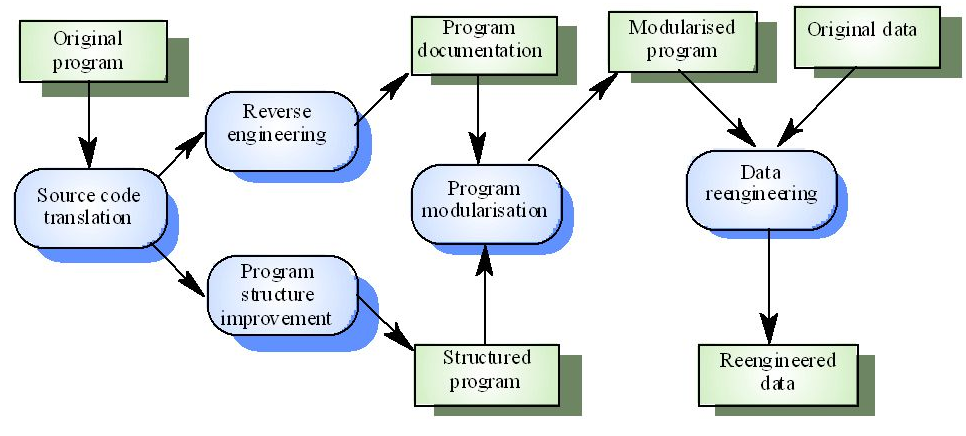
\includegraphics[scale=0.7]{re-engineering}
\end{center}
\subsection{Refactoring vs re-engineering}
Refactoring is a continuous process of improvement throughout the development and evolution process. It is intended to avoid the structure and code degradation that increases the costs and difficulties of maintaining a system.\\
\\
Re-engineering takes place after a system has been maintained for some time and maintenance costs are increasing. You use automated tools to process and re-engineer a legacy system to create a new system that is more maintainable. 
\section{Legacy systems}
Multiple strategies for legacy systems:
\begin{itemize}
	\item Scrap the system completely
	\item Continue maintaining the system
	\item Transform the system by re-engineering to improve its maintainability
	\item Replace the system with a new system
\end{itemize}
\subsection{Legacy system categories}
{\renewcommand{\arraystretch}{2}
\begin{tabularx}{\textwidth}{|X|X|X|}
\hline
& Low quality & High quality\\
\hline
Low business value& Scrap the system & Replace with COTS, scrap or maintain\\
\hline
High business value& Re-engineer or replace& Continue in operation with maintenance\\
\hline
\end{tabularx}}

\end{document}